\subsection{Describing bedload fluctuations: Including correlations between particle motions} 
\label{sec:ancey2008}

\citet{Ancey2006a, Ancey2008} developed a more general birth-death model in order to describe the relatively heavy tailed bedload probability distributions seen in experiments. 
In the last ten years, this model has been restated and more deeply studied by several authors \citep{Turowski2010, Heyman2013, Heyman2014a, Heyman2014, Ma2014}, and has led into exciting generalizations \citep{Turowski2010, Ancey2014, Ancey2015}. 
These are the real focus of this review. 

Instead of considering the motion of every bedload particle as an independent process involving transitions between motion and rest states, and summing a collection of these to get the total number of moving particles within the control volume, \citet{Ancey2008} consider the total number of moving particles within the control volume as a state.
In this case, instead of just two states (motion and rest), there is an infinite ladder of states ($n = 0,1,2 \dots$), each representing the number of active particles within the control volume.
The ladder of states is illustrated diagramatically in figure \ref{fig:ladder}. 

The advantage of this approach is when all particles are treated simulatenously, the transition rates can be made to depend on the number of active particles. 
The state is a collective property of the moving particles within the control volume. 
This allows interactions between particles to be introduced. 
\citet{Ancey2008} considers the population of moving particles changes due to entrainment (birth) and deposition (death), as before, but they also introduce migration processes for particles to move into (emigration) and out of (immigration) the control volume.
We note that these migration processes do not fundamentally modify the structure of the equations which result.
However, they are physically expected, so their inclusion is rational.

\begin{wrapfigure}{r}{0.5\textwidth}
  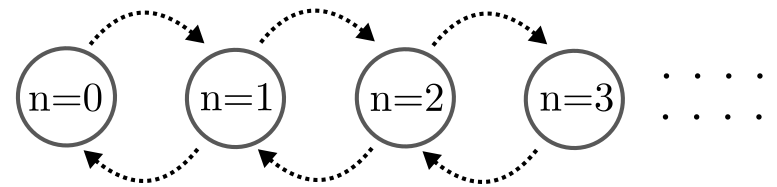
\includegraphics[width=.98\linewidth]{./figures/ancey2008.png}
  \caption{Birth, death, immigration, and emigration rates characterize the flow of probability up and down an infinite ladder of states. Each state represents $n$ particles in motion, and $n$ runs across all positive integers including zero. \label{fig:ladder} }
\end{wrapfigure} 

The key result of \citet{Ancey2008} is a successful description of wide bedload fluctuations. 
To obtain this, they made a component of the entrainment rate increase with the number of active particles. 
In effect, they introduced a positive feedback on entrainment: when more particles are in motion, entrainment becomes more likely. 
They termed this feedback term "collective entrainment".
The collective entrainment term fundamentally modifies the probability distribution of the bedload flux and lends it a wide tail, so the model is capable of describing realistically large fluctuations. 
Rather than a binomial distribution of the number of moving particles, as in \ref{eq:anceybinomial}, \citet{Ancey2008} derive a negative binomial distribution.
Within their model, collective entrainment is the source of the difference between these two distributions. 
When it is turned off, \citet{Ancey2008} reduces to \citet{Ancey2006}.  

Collective entrainment has been attributed to several physical mechanisms. 
Usually, the feedback is considered due to collisions of moving particles with the bed \citep{Ancey2008, Heyman2013, Heyman2014a} and the advection of turbulent structures implying waves of entrainment \citep{Ancey2008, Heyman2014}. 
Another consideration is that collective entrainment is the result of small avalanches, or local rearrangements of the bed surface triggered by the entrainment of an individual particle \citep{Heyman2014, Heyman2014a}. 
Entraining one grain could destabilize all of those contingent on it, so local microstructure \citep{Staron2006} may imply collective entrainment.  
These mechanisms for the collective entrainment term are reasonable, but they only hypotheses at this stage, and research is needed. 

The layout of this section is as follows: 
First, I will follow \citet{Ancey2008} to develop a master equation for the number $n$ of active particles within the control volume, obtaining a probability distribution $P(n)$. 
Then we can analyze the mean and variance of $n$ and develop the linkage to the probability distribution of the bedload flux, $P(q_s)$ using the relationship between volume and surface definitions of the flux, equation \ref{eq:fluxy}. 
This flux will be shown to link back to \citet{Einstein1950} as a limiting case. 
The magnitude of fluctuations will be considered, and we will conclude by a discussion of the model's assumptions and successes. 
In subsequent sections, we will examine generalizations of and other ways to study this model. 

\subsubsection{Master equation of the collective entrainment model} 

Consider the probability that there are $n$ particles in motion at time $t$. 
This can be denoted $P(n,t)$. 
The random variable $n$ takes on values $0,1,2,\dots$ -- non-negative integers of arbitrary magnitude. 
Each of these states has an associated probability $p_n(t)$.  
The population is subject to four transitions within a small time increment $\delta t$: 
\begin{enumerate}
\item 
Entrainment of a single bed particle (birth) can happen in time $\delta t$ with probability $\lambda_0 + \mu n$. 
The second term $\mu n$ is the collective entrainment effect. 
As the number of active particles increases, so does the rate of entrainment. 
This interaction term induces realistically wide bedload fluctuations. 
\item 
Deposition of a single bed particle can happen in $\delta t$ with probability $\sigma n$. 
This is similar to the telegrapher's process considered earlier. The rate of deposition increases with the number of active particles, just as it does implicitly in \citet{Ancey2006}. 
The deposition of each particle is independent of every other.  
\item 
Immigration of a particle from upstream into the control volume can happen in $\delta t$ with probability $\lambda_1$. 
This term does not fundamentally modify the structure of the equations we will derive for the probability distribution of the bedload rate. 
\item 
Emigration of a particle from the control volume to downstream can happen with probability $\nu$. 
This term is significant because it defines a bedload flux across a surface as in $q_s = \int dS \textbf{k} \cdot \textbf{u}_s$. 
Counting emigration events provides an alternate definition of the flux. 
This counting problem was solved by \citet{Ma2014}. 
We will consider this later. 
In this section, we will continue to interpret the flux as in section \ref{sec:fluxdef}, by converting an ensemble average to a volume average.
\end{enumerate} 
These transitions are depicted in figure \ref{fig:anceywindow}. 
The symbols of \ref{sec:ancey2008} are summarized in table \ref{tab:symbols2008}. 

\begin{wrapfigure}{l}{0.5\textwidth}
  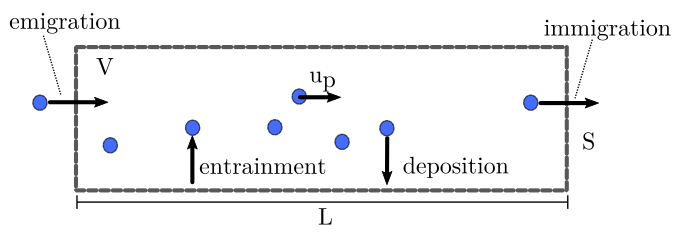
\includegraphics[width=.98\linewidth]{./figures/controlvol.png}
  \caption{As before, the model is based on analyzing the number of particles within a control volume $V$ which has downstream length $L$. Particles appear into the control volume due to entrainment and emigration. They disappear due to deposition and immigration. The downstream boundary is a stream cross section $S$.  \label{fig:anceywindow} }
\end{wrapfigure} 

We can consider the flow of probability up and down the ladder of states ($n=0,1,2,\dots$) which is induced by these transitions, entrainment (including the collective entrainment term), deposition, immigration, and emigration, using the formalism of more general Markov birth-death processes \citep{Cox1965, Pielou1977}. 
By the standard way of developing master equations \citep[e.g.][]{Cox1965}, we find an infinite system of equations for the probabilities of finding $n$ moving particles within the control volume: 
\begin{multline} P(n,t+\delta t) = \alpha \delta t (n+1)P(n+1,t) \\+  [\lambda + (n-1)\mu]\delta t P(n-1,t) \\ + [1-\delta t[\lambda + n\alpha + n\mu]]P(n,t). \label{eq:ancey2008master}\end{multline}
Here $\alpha = \nu + \sigma$ summarizes the contributions of emigration and deposition, which both act to decrease the number of particles $n$, and $\lambda = \lambda_0 + \lambda_1$ summarizes the contributions of immigration and (individual) entrainment, which both act to increase the number of particles $n$. 

As $\delta t\rightarrow 0$ these equations become a hirearchy of differential-difference equations for the probabilities $P(n,t)$ of finding $n$ particles in the control volume at time $t$: 
\be \frac{d}{dt}P(n,t) = (n+1) \alpha P(n+1,t) + [\lambda + (n-1)\mu]P(n-1,t) - [\lambda +n (\alpha+\mu)]P(n,t). \label{eq:anc2008} \ee 

These master equations define a birth-death immigration emigration model \citep[e.g.][]{Cox1965, Gardiner1983}. 
It can be solved for the probabilities $P(n,t)$ by introducing the probability generating function $G(z,t) = \sum_{n=0}^\infty z^n P(n,t)$ \citep{Cox1965, Gardiner1983, Ancey2008}. 
Multiplying \ref{eq:anc2008} by $z^n$ and summing over all $n$ gives, after a careful manipulation of the sums in order to form some function of $G(z,t)$ in every term, 
\be \frac{\partial}{\partial t} G(z,t) = \lambda(z-1)G(z,t) + \{ \sigma + \mu z^2 + \nu - (\mu + \sigma + \nu)z\} \frac{\partial}{\partial z} G(z,t). \ee

In effect, the probability generating function exchanges the discrete variable $n$ for a continous variable $z$. 
This first order partial differential equation for $G$ can be solved by the method of characteristics \citep{Cox1965, Garabedian1964}. 
If there are initially $N_0$ moving particles within the control volume, the solution is 
\be G(z,t) = \Big(\frac{\alpha-\mu}{(K-1)\mu z + \alpha - K \mu}\Big)^{n+\lambda/\mu}\Big( \frac{(K\alpha-\mu)z + \alpha(1-K)}{\alpha-\mu}\Big)^n. \label{eq:generator}\ee
The factor $K$ is the autocorrelation function $K(t) = \exp(-t(\alpha-\mu)).$

A useful feature of the probability generating function is that it generates the hirearchy of probabilities $P(n,t)$ via the Taylor expansion around $z=0$: $G(z,t) = \sum_{n=0}^\infty \frac{z^n}{n!}\big(\frac{\partial}{\partial z}\big)^n G(z,t) |_{z=0}$ \citep{Cox1965}. Comparing this formula with the definition of $G$, $G(z,t) = \sum_{n=0}^\infty z^n P(n,t)$, the coefficient of $z^n$ in the power series expansion of $G(z,t)$ is  apparently $P(n,t)$. 
The generating function provides the probability of finding $n$ particles in the control volume. 

Sufficiently far from the intial time, when $K(t) \approx 0 $ in the expression of $G$, meaning $t$ is much larger than the autocorrelation time $(\alpha-\mu)^{-1}$ so the system has forgotten its initial condition, the power series expansion of $G(z,t) \rightarrow G(z)$ generates a set of stationary probabilities for the number of bedload particles in motion within the control volume: 
\be P(n) = \frac{\Gamma(r+n)}{\Gamma(r)\Gamma(1+n)} p^r (1-p)^n\text{, }n=0,1,\dots. \label{eq:negbin0}\ee
Here $r=\lambda/\mu$ and $p = 1-\mu/\alpha$ characterize the strength of the collective entrainment factor $\mu$ relative to the other transitions which act to increase ($\lambda$) or decrease ($\alpha$) the population.  
$\Gamma(x) = \int_0^\infty z ^{x-1} e^{-z} dz$ is the well-known $\Gamma$ function of mathematical physics \citep{Boas2005, Mathews1971}. It is a generalization of $x!$ to non-integer values of $x$. 
This stationary distribution only exists when $\alpha>\mu$: the rate at which sediment particles appear in the control volume is lower than their disappearance rate. 
The set of symbols introduced in the \citet{Ancey2008} formulation is summarized in table \ref{tab:symbols2008}. 

\begin{wraptable}{l}{0.5\linewidth}
\vspace{-10pt}
\caption{The parameters used in section \ref{sec:ancey2008}}\label{tab:symbols2008}
\begin{tabular}{p{3.3cm}p{3.3cm}}\\
\toprule  
Symbol & Meaning \\
\midrule
$\nu$ & emigration  \\  
$\sigma$ & deposition \\  
$\lambda_0$ & immigration  \\ 
$\mu$ & collective entrainment\\
$\lambda_1$ & entrainment\\ 
$\lambda$ &  $\lambda_0 + \lambda_1$ \\ 
$\alpha $& $\sigma+\nu$ \\
$r$ & $\lambda/\mu$ \\
$p$ & $1-\mu/\alpha$ \\
\bottomrule
\end{tabular}
\end{wraptable} 

This stationary distribution equation \ref{eq:negbin0} is the negative binomial distribution: 
\be P(n) \sim \text{NegBin}(r,p).\label{eq:negbin}\ee
It is a generalization of the binomial distribution for the number of active particles, equation \ref{eq:anceybinomial}, which was derived in the \citet{Ancey2006} paper.
The negative binomial distribution has a relatively heavy tail, so that large deviations in the number of active particles $n$ are possible. 
These large fluctuations are the result of the collective entrainment rate $\mu$, and they allow the birth-death immigration-emigration model to express bedload fluctuations of realistic magnitude. 
As we will show, they become relatively small as collective entrainment is turned off, $\mu \rightarrow 0$. 

\subsubsection{The bedload flux: wide fluctuations and the Einstein limit}

As discussed, the negative binomial distribution supports wide fluctuations, controlled by the collective entrainment parameter $\mu$. 
The mean number of particles in the control volume, taken over the distribution \ref{eq:negbin}, is 
\be \bra n \ket = \sum_{n=0}^\infty n P(n) = \frac{\lambda \alpha}{\alpha-\mu}. \label{eq:anceymean}\ee
Likewise the variance is 
\be \bra \delta n^2 \ket = \sum_{n=0}^\infty (n-\bra n\ket)^2 P(n) = \frac{ \lambda \alpha}{\alpha-\mu^2},\ee
which means their ratio is 
\be \frac{\bra \delta n^2\ket }{\bra n\ket} = \frac{1}{1-\mu/\alpha}.\ee
It is interesting to compare this to equation \ref{eq:2006flucts} bounding the magnitude of fluctuations in the \citet{Ancey2006} model. 
In contrast, within the \citet{Ancey2008} model, the variance must exceed the mean, because as discussed, in steady state $\alpha>\mu$. 
The magnitude of fluctuations can grow arbitrarily with the collective entrainment parameter $\mu$. 
This is a coherent conclusion, since collective entrainment was introduced in order to represent the collective effects of turbulent fluctuations, collision-induced entrainment, and granular avalanches; and with the expressed intent of generating realistically wide bedload fluctuations, exceeding those of the \citet{Ancey2006} model. 

Armed with the probability distribution for the number of particles in the control volume, equation \ref{eq:negbin}, and the link between control volume and surface statistics derived in section \ref{sec:fluxdef}, equation \ref{eq:fluxy}, we can derive the probability distribution of the bedload flux in a similar way as equation \ref{eq:anceygauss}.
Using the law for transformation of probabilities gives 
\be P(q_s) \approx \frac{\Gamma(r+\frac{Lw}{\nu_p u_s} q_s)}{\Gamma(r)\Gamma(1+\frac{Lw}{\nu_p u_s} q_s)}p^r(1-p)^{\frac{Lw}{\nu_p u_s} q_s}\ee
as the probability distribution of the bedload flux $q_s$.
The bedload flux, as derived in \citet{Ancey2008}, is a random variable with a negative binomial distribution.  

Now we link back to the \citet{Einstein1950} theory. 
Einstein considered neither immigration ($\lambda_0$), emigration ($\nu$), nor collective entrainment ($\mu$). 
When all of these parameters are set to zero, $\mu = \lambda_0 = \nu = 0$, the parameters $r$ and $p$ of the distribution \ref{eq:negbin0} become $r \rightarrow \infty$ and $p=0$. 
With these limits, the distribution \ref{eq:negbin0} tends to a Poisson distribution. 
There are several ways to show this. 
The simplest way is to take the appropriate limits ($t \rightarrow \infty$, $\mu=\lambda_1=\nu= 0$)  into the generating function \ref{eq:generator}, giving
\be G(z) = e^{-\lambda_0(z-1)/\sigma}.\ee
This inverts to ($P(n) = \frac{1}{n!}(\partial/\partial z)^n G(z)|_{z=1}$)
\be P(n) = \frac{(\lambda_1/\sigma)^n}{n!}e^{-\lambda_1/\sigma},\label{eq:anceypoisson}\ee
the Poisson distribution with rate $\lambda_0/\sigma$.
The \citet{Ancey2008} model links to the limiting result of \citet{Ancey2006}, equation \ref{eq:ancey2006limit2}. 

Using equation \ref{eq:fluxy} with this Poisson distribution, equation \ref{eq:anceypoisson}, we compute the number of active paricles $n$ in the absence of collective entrainment: 
\be \bra q_s \ket = \frac{\nu_p u_s}{L w} \sum_{n=0}^\infty n \frac{(\lambda_1/\sigma)^n}{n!}e^{-\lambda_1/\sigma} = \frac{\nu_p u_s}{L w} \frac{\lambda_1}{\sigma}. \label{eq:ancey2008mean}\ee
To connect equation \ref{eq:ancey2008mean} with the Einstein-like formula of Yalin, equation \ref{eq:yalinflux}, requires a delicate interpretation of the parameters $\lambda_0$ and $\sigma$. 
The rate of entrainment $\lambda_1$ pertains to all particles within the control volume, of which there is a very large number $N \rightarrow \infty$. 
Meanwhile, the rate of deposition $\sigma$ pertains to an individual particle. 
These interpretations are consistent with the master equation \ref{eq:ancey2008master}. 
Hence if we define the probability that (only) one particle entrains in a small interval $\delta t$ as $\lambda'$, then $\lambda = N\lambda'$, and the mean flux is 
\be \bra q_s \ket = \frac{\nu_p u_s}{L w}\frac{N\lambda'}{\sigma}.\ee
If we can again interpret the ratio $N/(Lw)$ as proportional to the area of an individual particle, using $\nu_p \propto a^3$, and the travel distance $l\propto a$, we get 
\be \bra q_s \ket = A \frac{a l}{a/u_s}\frac{\lambda'}{\sigma}, \ee
again in accord with the Yalin result \ref{eq:yalinflux}. 

We have shown that the assumptions of \citet{Einstein1950} can be mixed with stochastic mathematics to develop a more coherent and physically-based theory of the bedload flux, as performed by \citet{Ancey2006}. 
Since the fluctuations predicted by the Gaussian bedload flux of \citet{Ancey2006} are not sufficiently large to describe experiments, we have mimiced \citet{Ancey2008} to include collective motion effects in order to express bedload fluctuations of sufficient magnitude from a birth-death model. 
Turning off the extra processes in the \citet{Ancey2008} model leads to a coherent connection back to a limiting result of \citet{Ancey2006}, and further to back to Yalin's revision of Einstein \citep{Yalin1972}. 

However, there is obviously some ambiguity around the number of particles available for motion, which was denoted $N$ in previous sections in this review. 
Apparently, the \citet{Ancey2008} model considers the $N\rightarrow \infty$ limit, while the probability that any one particle is observed in motion goes to zero, similar to the Poisson limit of the \citet{Ancey2006} model. 
Of course, the number of particles available for motion is not unlimited. 
Over a purely alluvial bed composed to gravel, it must be limited by the number of particles on the bed surface. 
Within the idealization of \citet{Einstein1950}, this constraint was expressed by the equation $N a^2 \propto Lw$. 

In the collective model of \citet{Ancey2008}, limiting the number of particles available for motion is more difficult. 
The most obvious way would be to consider that the entrainment rate of all particles is proportional to the entrainment rate of a single particle, times the number of particles at rest, such as $\lambda'(N-n)$. 
However, this does not work because particles can also arrive from upstream, meaning $n$ can exceed $N$. 
In this case, to consider the rate of entrainment decreases with the number of active particles, one would need to disciminate how the particles got into the control volume in the first place. 
Did they entrain, or did they emigrate?
This is non-Markovian. 
A second way to impose that a finite number of bed particles are available for entrainment is to consider the Markovian dynamics of two species at once: the bed surface particles, and the particles in motion. 
This path was taken by \citet{Turowski2009}, and this is the next section of the review. 
